\let\negmedspace\undefined
\let\negthickspace\undefined
\documentclass[journal]{IEEEtran}
\usepackage[a5paper, margin=10mm, onecolumn]{geometry}
\usepackage{lmodern}
\usepackage{tfrupee} % Include tfrupee package

\setlength{\headheight}{1cm}
\setlength{\headsep}{0mm}
\usepackage{gvv-book}
\usepackage{gvv}
\usepackage{algorithmicx} % Ensure algorithmicx is loaded explicitly
\usepackage{cite}
\usepackage{amsmath,amssymb,amsfonts,amsthm}

\usepackage{graphicx}
\usepackage{textcomp}
\usepackage{xcolor}
\usepackage{txfonts}
\usepackage{listings}
\usepackage{enumitem}
\usepackage{mathtools}
\usepackage{gensymb}
\usepackage{comment}
\usepackage[breaklinks=true]{hyperref}
\usepackage{tkz-euclide} 
\usepackage{listings}                                       
\def\inputGnumericTable{}                                  
\usepackage[latin1]{inputenc}                               
\usepackage{color}                                          
\usepackage{array}                                          
\usepackage{longtable}
\usepackage{multicol}
\usepackage{calc}                                           
\usepackage{multirow}                                        
\usepackage{hhline}                                          
\usepackage{ifthen}                                          
\usepackage{lscape}
\usepackage{algorithm}
\usepackage{algpseudocode}

\renewcommand{\thefigure}{\theenumi}
\renewcommand{\thetable}{\theenumi}
\setlength{\intextsep}{10pt}

\numberwithin{equation}{enumi}
\numberwithin{figure}{enumi}
\renewcommand{\thetable}{\theenumi}

\begin{document}

\bibliographystyle{IEEEtran}
\vspace{3cm}

\title{11.16.2.2.2}
\author{EE24BTECH11011 - Pranay Kumar}
\maketitle

\textbf{Question}:\\
A die is thrown. Describe the following event:
(i) $ A $: A number less than 7.\\
(ii) $ B $: A number greater than 7.

Also, find the following Boolean operations: 
$ A \lor B, A \land B$

\textbf{Solution: }\\

\textbf{Textual solution: }\\
Event $ A $ represents outcomes less than 7. Since a fair die has outcomes $\{1, 2, 3, 4, 5, 6\}$, this event includes all possible outcomes:
\begin{align}
    A &= \{1, 2, 3, 4, 5, 6\}.
\end{align}
The probability of event $ A $ occurring is:
\begin{align}
    P(A) &= \frac{|A|}{6} = \frac{6}{6} = 1.
\end{align}

Event $ B $ represents outcomes greater than 7. Since a fair die has outcomes $\{1, 2, 3, 4, 5, 6\}$, this event is impossible:
\begin{align}
    B = \emptyset, \quad P(B) = 0.
\end{align}

Using Boolean operations:
\begin{align}
    A \lor B &= A, \\
    A \land B &= \emptyset.
\end{align}

\textbf{Additional Analysis Using A and B: }\\
Since $ B $ is an impossible event:
\begin{align}
    P(A \lor B) &= P(A) + P(B) - P(A \land B) = P(A) + 0 - 0 = P(A), \\
    P(A \land B) &= 0.
\end{align}

Since $ A $ includes all possible outcomes of a fair die:
\begin{align}
    P(A) &= 1.
\end{align}

Thus,
\begin{align}
    P(A \lor B) &= 1, \\
    P(A \land B) &= 0.
\end{align}

\textbf{Computational solution: }\\
\section*{Computation of Probabilities for Rolling a Die}
To verify the theoretical results, we perform a simulation by rolling a die $ N $ times and tracking outcomes.

\subsection*{Definitions}
\subsubsection*{Probability Mass Function (PMF)}
For a six-sided die:
\begin{align}
    P(X = k) = \frac{1}{6}, \quad k \in \{1,2,3,4,5,6\}.
\end{align}

\subsubsection*{Cumulative Distribution Function (CDF)}
\begin{align}
F(x) = \begin{cases} 
0, & x < 1, \\
\frac{x}{6}, & x \in \{1,2,3,4,5,6\}, \\
1, & x > 6.
\end{cases}
\end{align}

The probability $ P(B) $ is computed as:
\begin{align}
    P(B) = 1 - F(6) = 1 - 1 = 0.
\end{align}

\subsection*{Calculation of Boolean Operations}
Using simulated data, we compute probabilities:
\begin{align}
    P(A \lor B) &= P(A) = 1, \\
    P(A \land B) &= 0. \\
\end{align}

\subsection*{Simulation Process}
We roll a die $ N $ times and compute probabilities empirically. The following steps outline the process:
\begin{enumerate}
    \item Simulating Outcomes: A random integer $ X $ is generated for each trial, where $ X \in \{1, 2, 3, 4, 5, 6\} $.
    \item Tracking Occurrences: For each simulated roll, the number of occurrences of each outcome is tracked.
    \item Computing PMF: The PMF is computed by dividing occurrences by $ N $.
    \item Computing CDF: The CDF is derived from the PMF.
    \item Verifying Theoretical Probability.
\end{enumerate}

\subsection*{Output Representation}
\begin{figure}[h!]
    \centering
    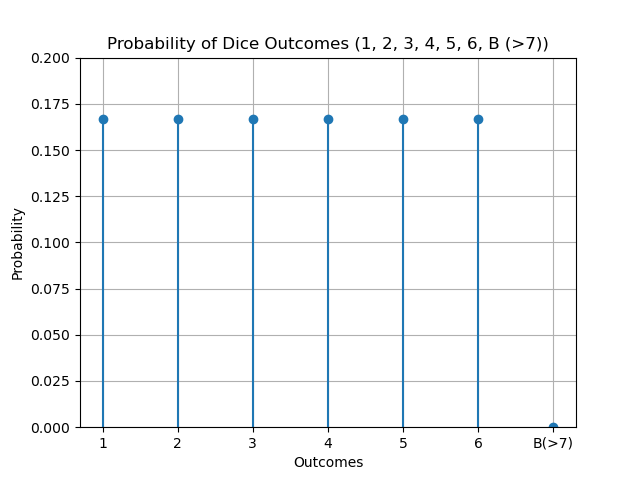
\includegraphics[width=\columnwidth]{figs/fig.png}
    \caption{Probability analysis of dice roll events}
    \label{fig:event_probs}
\end{figure}

\end{document}

